%************************************************
\chapter{Systembeschreibung und Analysemethode}\label{kap:systembeschreibung}
%************************************************

Dieses Kapitel gliedert sich in zwei Teile. Im ersten Teil werden zum Zweck der Vergleichbarkeit die Rahmenbedingungen der in \autoref{kap:simulation} beschriebenen Simulation festgelegt, der zweite Teil beschäftigt sich mit der Analysemethode und definiert Messgrößen für die spätere Bewertung der Ergebnisse.

\section{Ein geeignetes Szenario}
\begin{figure}[bth]
        \myfloatalign
        {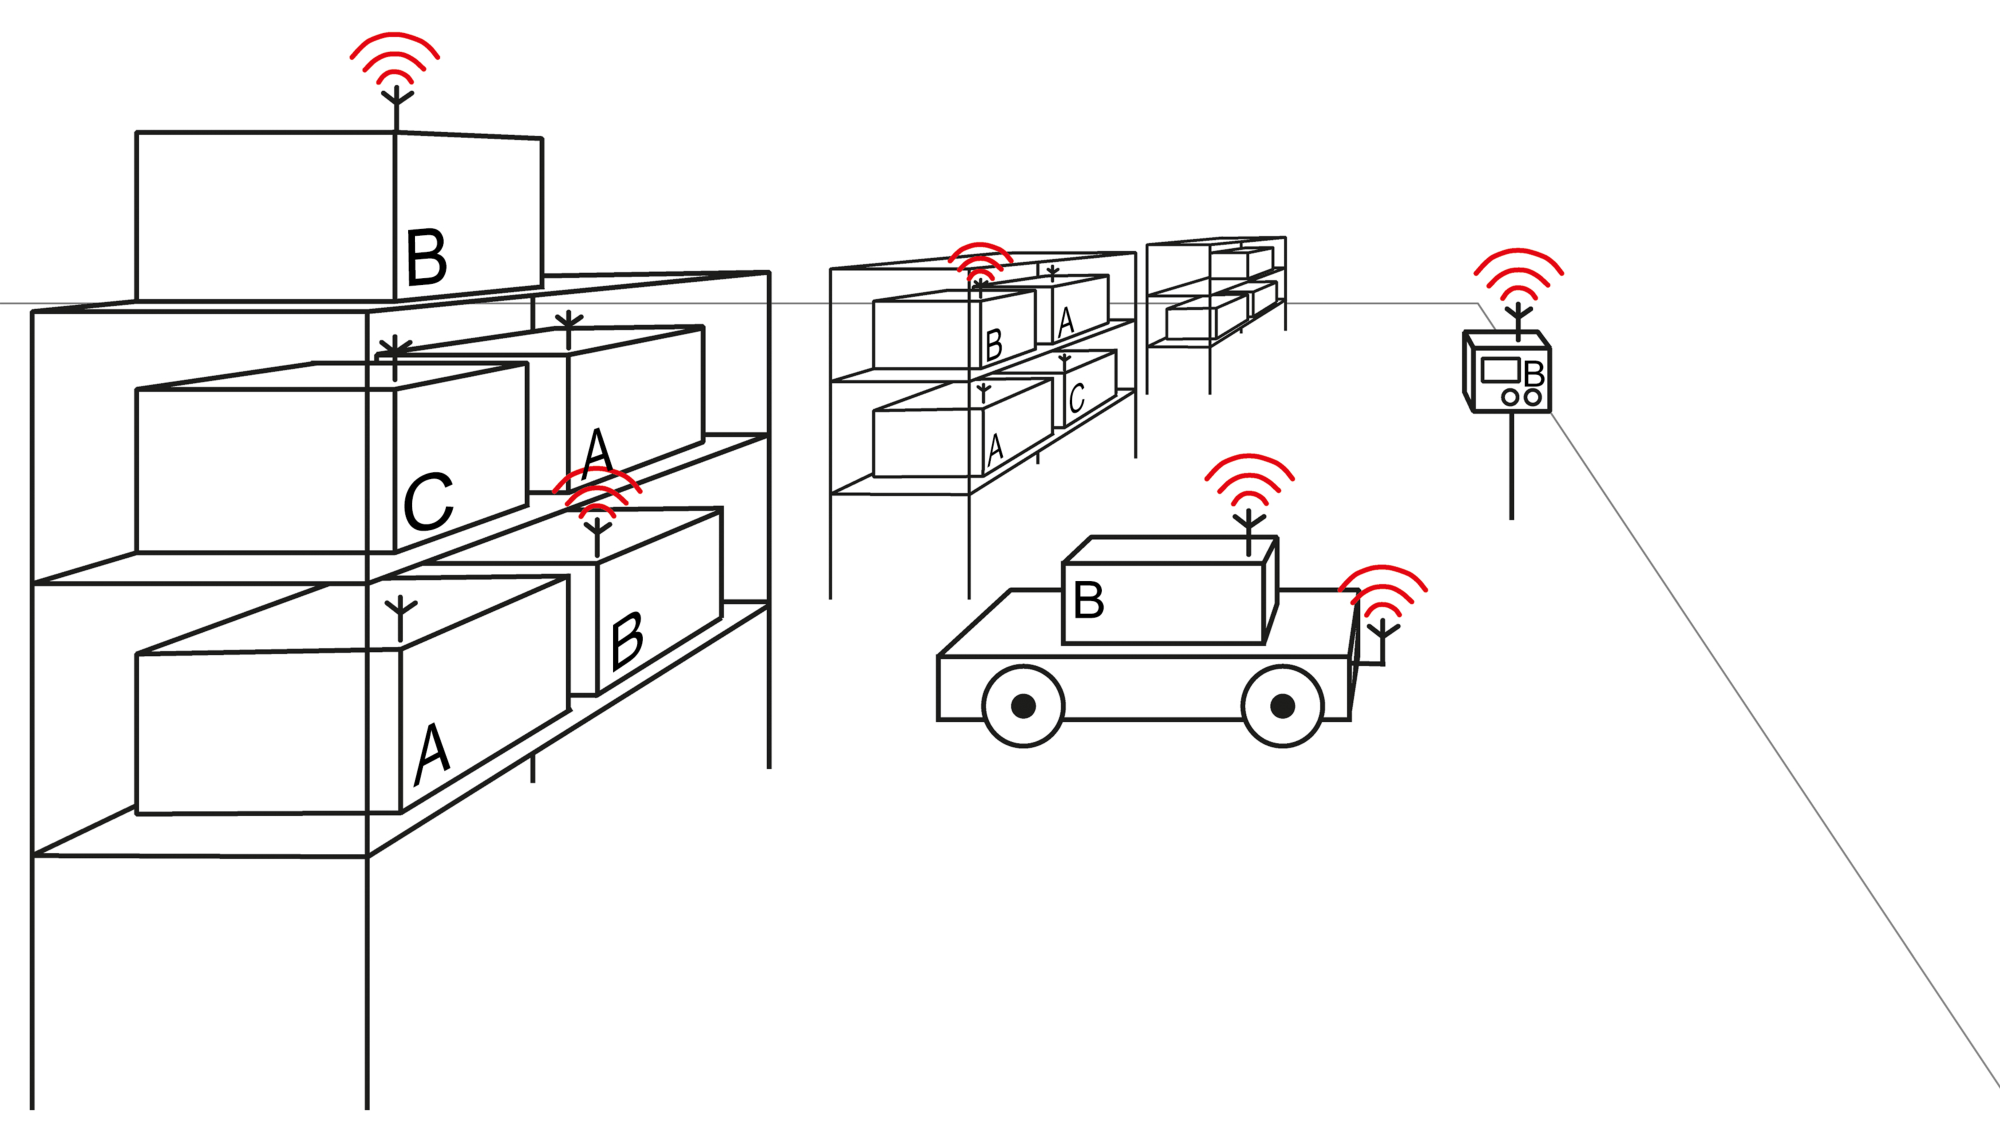
\includegraphics[width=1\linewidth]{gfx/uebersicht}} 
        \caption[Scenario]{Andeutung des Logostikszenarios mit vernetzten Frachtcontainern}\label{fig:lageruebersicht}
\end{figure}
Hauptbestandteil eines intelligenten Logistiklagers sind die Frachtcontainer mit den verschiedenen Gütern. Daneben gibt es Systeme zur Beförderung und Einlagerung der Frachtcontainer, dafür können auch mobile Roboter zu Einsatz kommen, wie in \autoref{fig:lageruebersicht} angedeutet. Dienstprogramme, wie eine automatische Inventarisierung oder Kommissionierung, also das Zusammenstellen von bestimmten Produkten für einen Auftrag, gehören ebenfalls zu  einem selbst organisierten Warenlager. Sowohl die Systeme zur Beförderung als auch die Computer, auf denen die Dienstprogramme ausgeführt werden, müssen in der Lage sein, mit den Frachtcontainern zu kommunizieren. Sie werden damit Teil des Funknetzwerkes. Üblicherweise sind in einen Kommunikationsprozess die Container involviert, die das gleiche Produkt oder eine bestimmte Kategorie an Frachtgütern beinhalten. In \autoref{fig:lageruebersicht} hat \zB gerade ein Kommunikationsprozess bezogen auf das Produkt B begonnen. Charakteristisch ist, dass dabei eine Anfrage von einer Stelle ausgeht und für eine Vielzahl an Empfängern --- den Frachtcontainern --- bestimmt ist, die diese Anfrage beantworten. Von welcher Quelle genau die Anfrage stammt, ist für die Funktion des Kanalzugriffverfahren unerheblich, da sich immer o.g. Muster ergibt. Eine mobile Transporteinheit, die den kürzesten Weg zu einem Produkt finden möchte, oder eine Verfügbarkeitsanfrage über das Internet sind nur zwei Beispiele.

\subsection{Anordnung}
Als Grundlage für die spätere Simulation wird ein Anordnung angenommen, die der typischen Platzierung von Frachtcontainern in Logistiklagern entspricht. Dabei werden die Container in mehreren Zeilen von Hochregalen eingelagert, sodass sich die \glspl{node} des zu untersuchenden \ac{wsn} in einer dreidimensionalen Matrix befinden. 

\begin{figure}[bth]
        \myfloatalign
        {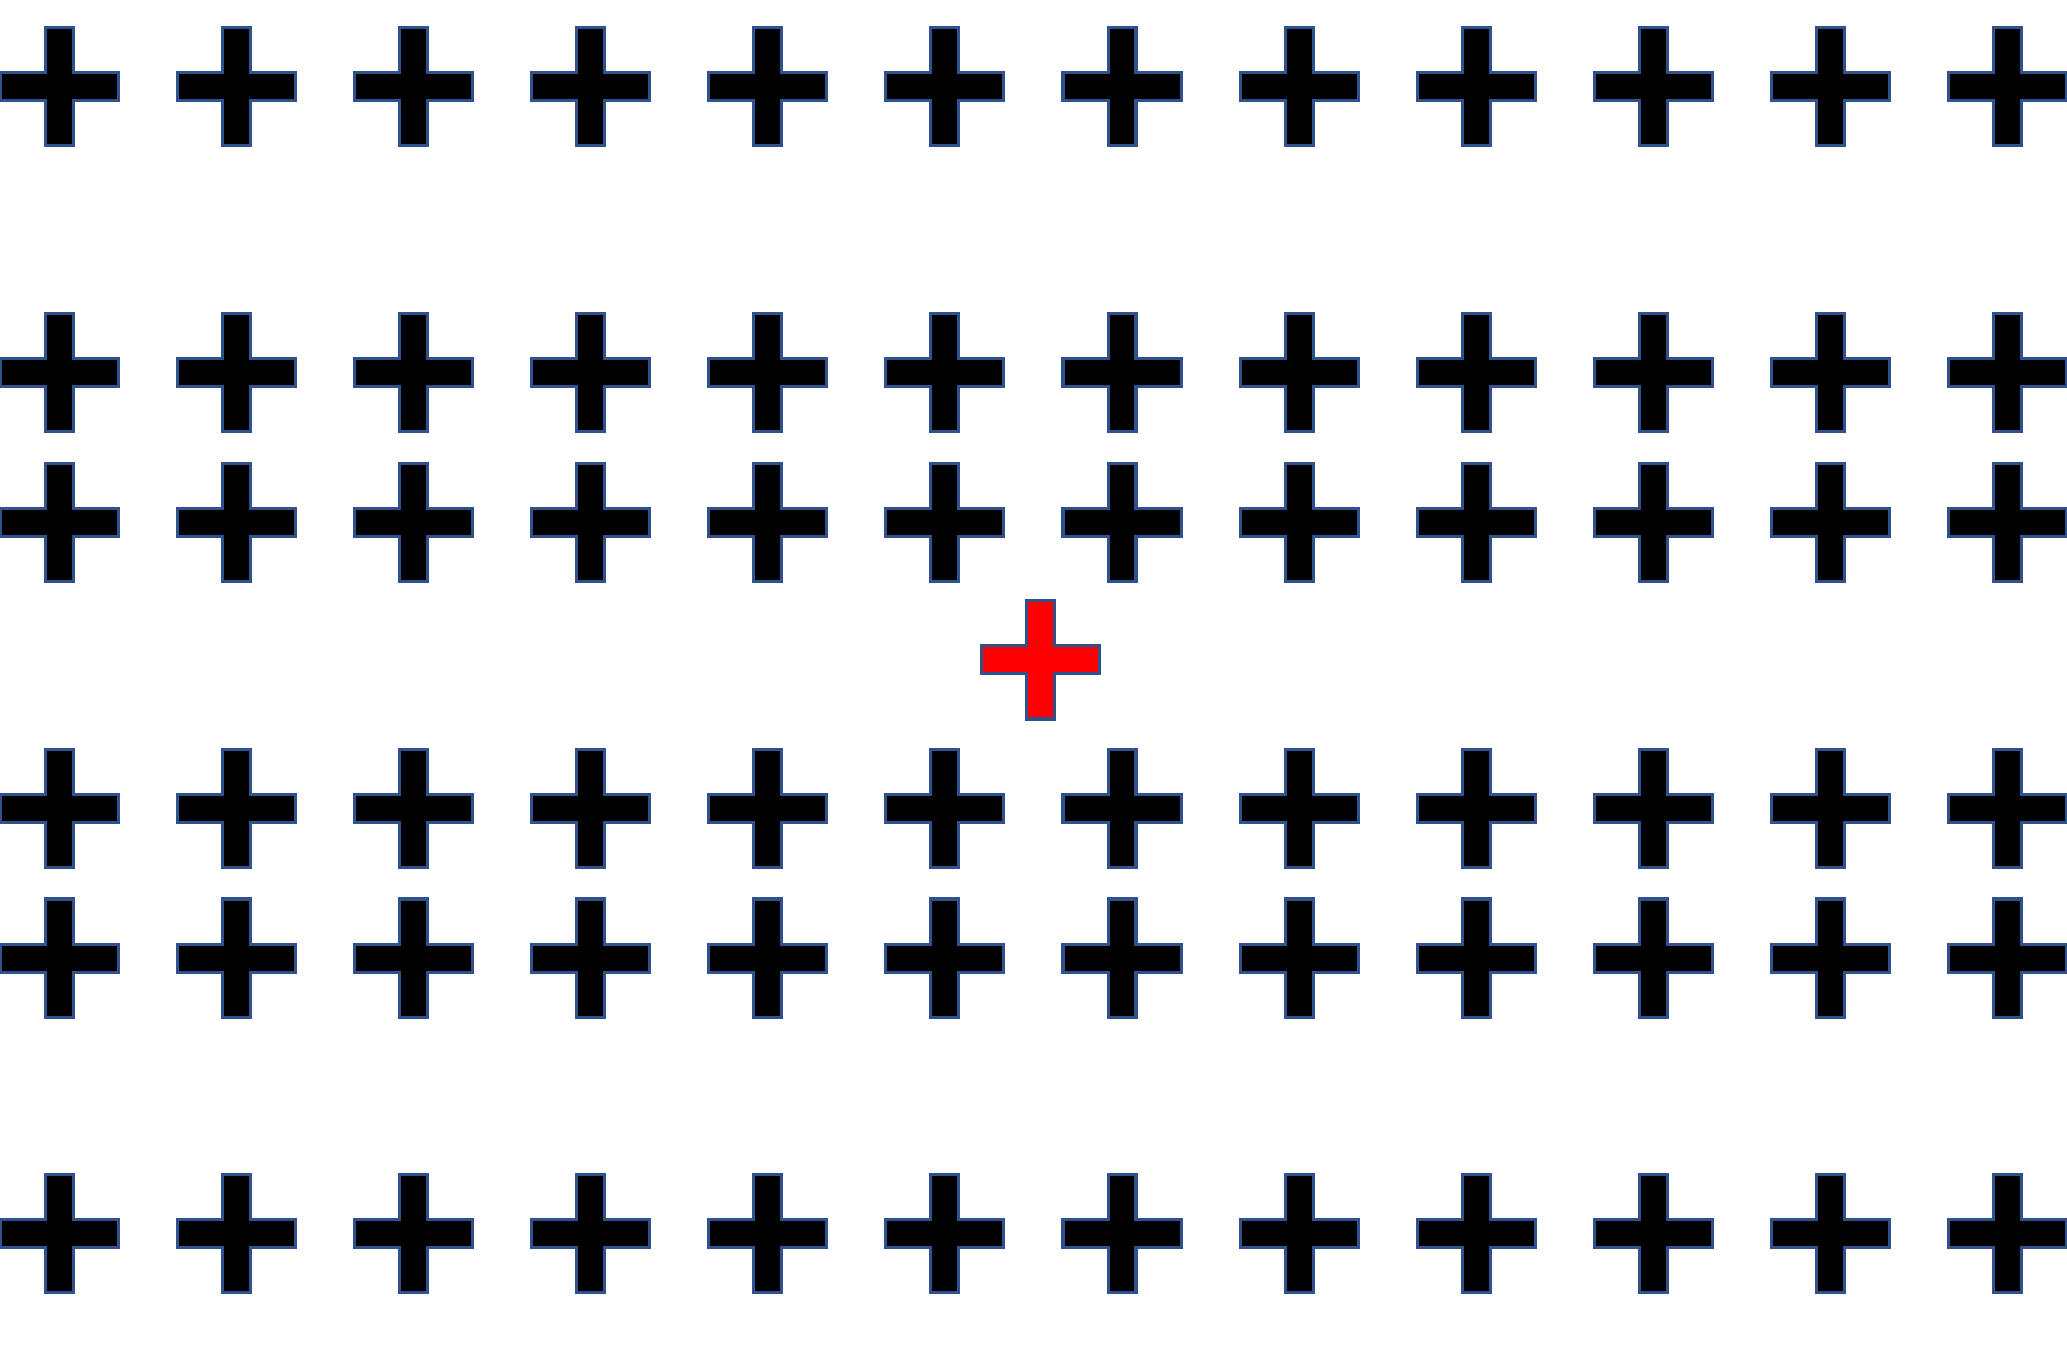
\includegraphics[width=0.4\linewidth]{gfx/anordnung}} 
        \caption[Anordnung von Frachtcontainern in einem Logistiklager]{Die einzelnen Frachtcontainer werden in einem Logistiklager in Hochregalen zeilenweise eingelagert. Die Grafik zeigt die Aufsicht der Containerpositionen. An der rot markierten Position befindet sich der \acs{ap}}\label{fig:lager}
\end{figure}

Weiterhin wird in dieser Arbeit angenommen, dass es einen einzelnen Funkknoten gibt dessen Reichweite das gesamte Lager abdeckt und im weiteren Verlauf dieser Arbeit als \ac{ap} bezeichnet wird. Eine Anordnung mit mehreren \acp{ap} zur Reduzierung der Sendeleistungen ist sinnvoll \citep{Falkenberg2017b}, jedoch hier nicht Gegenstand der Untersuchung. Die Beobachtungen hinsichtlich der Netzlast in dem hier gewählten Ansatz lassen sich unter Berücksichtigung von Überlappungen auf ein Szenario mit mehreren \acsp{ap} übertragen. \autoref{fig:lager} zeigt diese Anordnung aus der Aufsicht.

\subsection{Energieversorgung}
Für die spätere Bewertung der Energiebilanz wird angenommen, dass der \ac{ap} über eine unkritische Energieversorgung verfügt --- \zB direkt an das Stromnetz angeschlossen ist. Dagegen steht an den einzelnen \glspl{node} nur eine sehr begrenzte Menge an Energie zu Verfügung, mit der effizient zu haushalten ist \cite{inBin}.

\subsection{Datenaufkommen} \label{kap:systembeschreibung_sek:datenaufkommen}
Um die Paketgröße der ausgetauschten Nachrichten abzuschätzen, werden die folgenden Punkte berücksichtigt:
\begin{description}
	\item[Identifizierung des Frachtcontainers] Um einen Frachtcontainer zu identifizieren, ist eine eindeutige Adresse notwendig. Hier bietet sich die \ac{mac} Adresse an, die im  IEEE 802.15.4 Standard verwendet wird \cite{ieee}. Diese ist acht Byte lang \cite[151]{ieee}.
	\item[Identifikation des Frachtgutes] Wie in \citep{inBin} beschrieben, werden Güter in automatisierten Logistikprozessen mit der \acs{rfid}-Technologie identifiziert. Hierbei wird der \acf{epc} des Produkts ausgelesen. Zur Identifizierung eines einzelnen Produkts dient die \acf{gtin}, die typischerweise in einem Strichcode codiert ist. Da die  \acs{rfid}-Technologie aber auch das berührungslose Auslesen von größeren Gebinden erlaubt, enthält der \acs{epc} zusätzlich Informationen über die logistische Einheit, wie \zB Verpackungseinheit oder Palette. Der \acs{epc} besteht in der gebräuchlichsten Form aus 12 Byte \citep{epc}. 
	\item[Nachrichten Typ] Die unterschiedlichen Nachrichten-Arten können in einem Byte codiert werden. Das erlaubt theoretisch bis zu 256 verschiedene Nachrichtenarten oder das Verwenden von einzelnen Bits innerhalb dieses Bytes für Steuerinformationen, \zB Sequenznummern.
	\item[Parameter] Dieser Teil der Nachricht bietet Platz für zusätzliche Informationen je nach Nachrichtenart und wird pauschal mit zwei Byte veranschlagt.
\end{description}

Die genannten Punkte bilden die wesentlichen Bestandteile für den Informationsaustausch innerhalb eines Logistklagers. \autoref{tab:pktlen} gibt einen Überblick über die resultierende Paketlänge. Es wird hierbei davon ausgegangen, dass eine Nachricht in der Regel alle Felder, jedoch mindestens Nachrichten-Typ und ein weiteres Feld enthält. Daher wird in \autoref{fig:frame} ein Nachrichtenrahmen mit fester Länge definiert.

\begin{table}
    \myfloatalign
  \begin{tabularx}{0.7\textwidth}{Xll} \toprule
    \tableheadline{Feld} & \tableheadline{Länge in Byte} \\ \midrule
    Node ID $($\acs{mac}-Adresse$)$ & 8 \\
    Produkt ID $($\acs{epc}$)$ & 12 \\
    Nachrichten-Typ & 1 \\
    Parameter & 2 \\
    \midrule
    Summe & 23 \\
    \bottomrule
  \end{tabularx}
  \caption[Nachrichtenfelder]{Bestandteile einer exemplarischen Nachricht für die Kommunikation in Logistiklagern}  \label{tab:pktlen}
\end{table}

\begin{figure}[bth]
        \myfloatalign
        {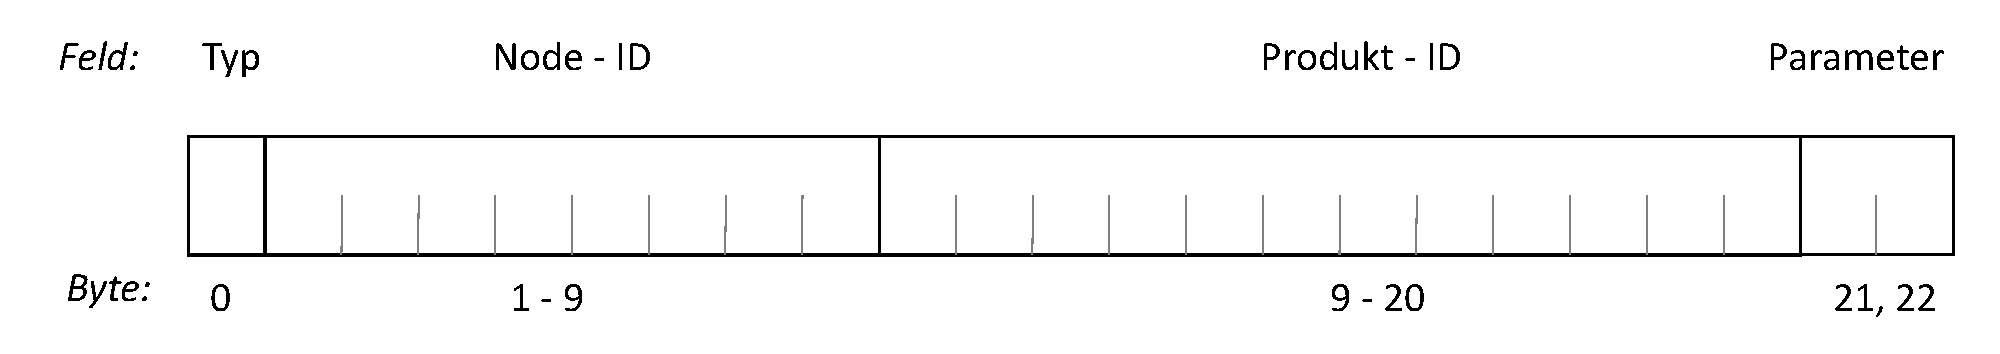
\includegraphics[width=1\linewidth]{gfx/Frame-Muster}} 
        \caption[Nachrichtenrahmen]{Nachrichtenrahmen mit fester Länge für den Informationsaustausch im Logistiklager}\label{fig:frame}
\end{figure}


\subsection{Kommunikationsfluss}
Die zwei Kernpunkte des Informationsaustausches für das zu untersuchende Szenario sind:
\begin{enumerate}
\item Anfragen nach einem bestimmten Produkt
\item Meldung der Frachtcontainer über deren Inhalt
\end{enumerate}
Darüber hinaus sind weitere Nachrichten zur Organisation nötig, wie etwa:
\begin{aenumerate}
\item Anmeldung neuer Frachtcontainer
\item Zuweisung eines Produktes zu einem Frachtcontainer
\item Meldung der Frachtcontainer über geringen Warenbestand
\item Fehlermeldungen
\end{aenumerate}
Für die Untersuchung eines leistungsfähigen Kanalzugriffprotokolls spielen diese Nachrichten jedoch eine untergeordnete Rolle. Die Erprobung des Kanlzugriffprotokolls bezieht sich auf einen \emph{Anfrage-Antwort} Zyklus, der vom \acs{ap} initiiert wird. Dazu werden in \autoref{fig:nachrichten} zwei Nachrichtentypen nach dem Schema aus \autoref{kap:systembeschreibung_sek:datenaufkommen} definiert. Der erste Typ ist \emph{PAGE} und dient der Anfrage nach einem Produkt, der zweite Typ heißt \emph{QUANTITY} und ist für die Antworten der Frachtcontainer vorgesehen. Die PAGE-Nachricht wird als Broadcast in das Netz geschickt und löst damit nahezu gleichzeitige QUANTITY-Nachrichten der \glspl{node} aus. Im Gegensatz zu \cite{inBinTestbed} wird von regelmäßigen Status-Nachrichten von Seiten der Frachtcontainer abgesehen. Der Ablauf eines Kommunikationszyklus ist in \autoref{fig:sequenz} als Sequenzdiagramm dargestellt.

\begin{figure}[bth]
        \myfloatalign
        \subfloat[Typ 1 Nachricht: PAGE]
        {\label{fig:nachrichten-a}%
         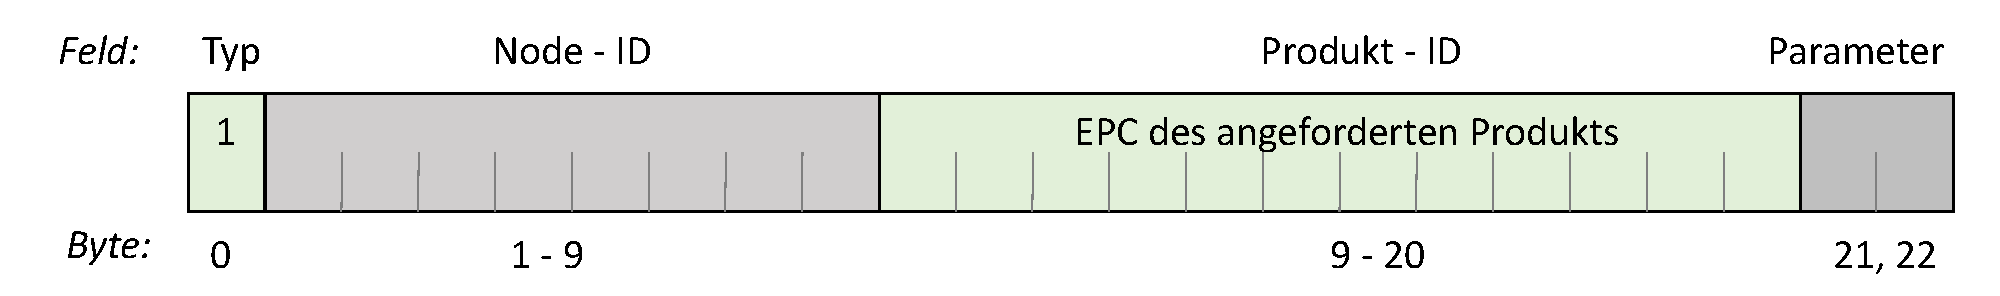
\includegraphics[width=1\linewidth]{gfx/Page-Frame}} \\
        \subfloat[Typ 2 Nachricht: QUANTITY]
        {\label{fig:nachrichten-b}%
        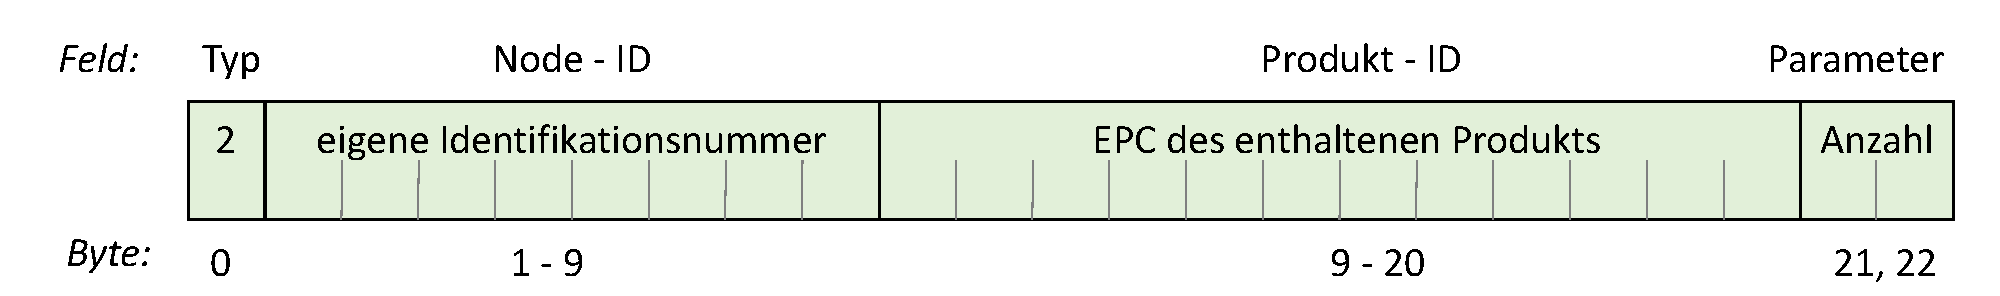
\includegraphics[width=1\linewidth]{gfx/Quantity-Frame}} 
        \caption[Nachrichtentypen]{Nachrichtentypen zur Abfrage von bestimmen Produkten. a) PAGE Nachricht mit angefordertem Produkt. b) QUANTITY Nachricht mit Anzahl der im Frachtcontainer verfügbaren Menge.}\label{fig:nachrichten}
\end{figure}

\begin{figure}[bth]
        \myfloatalign
        {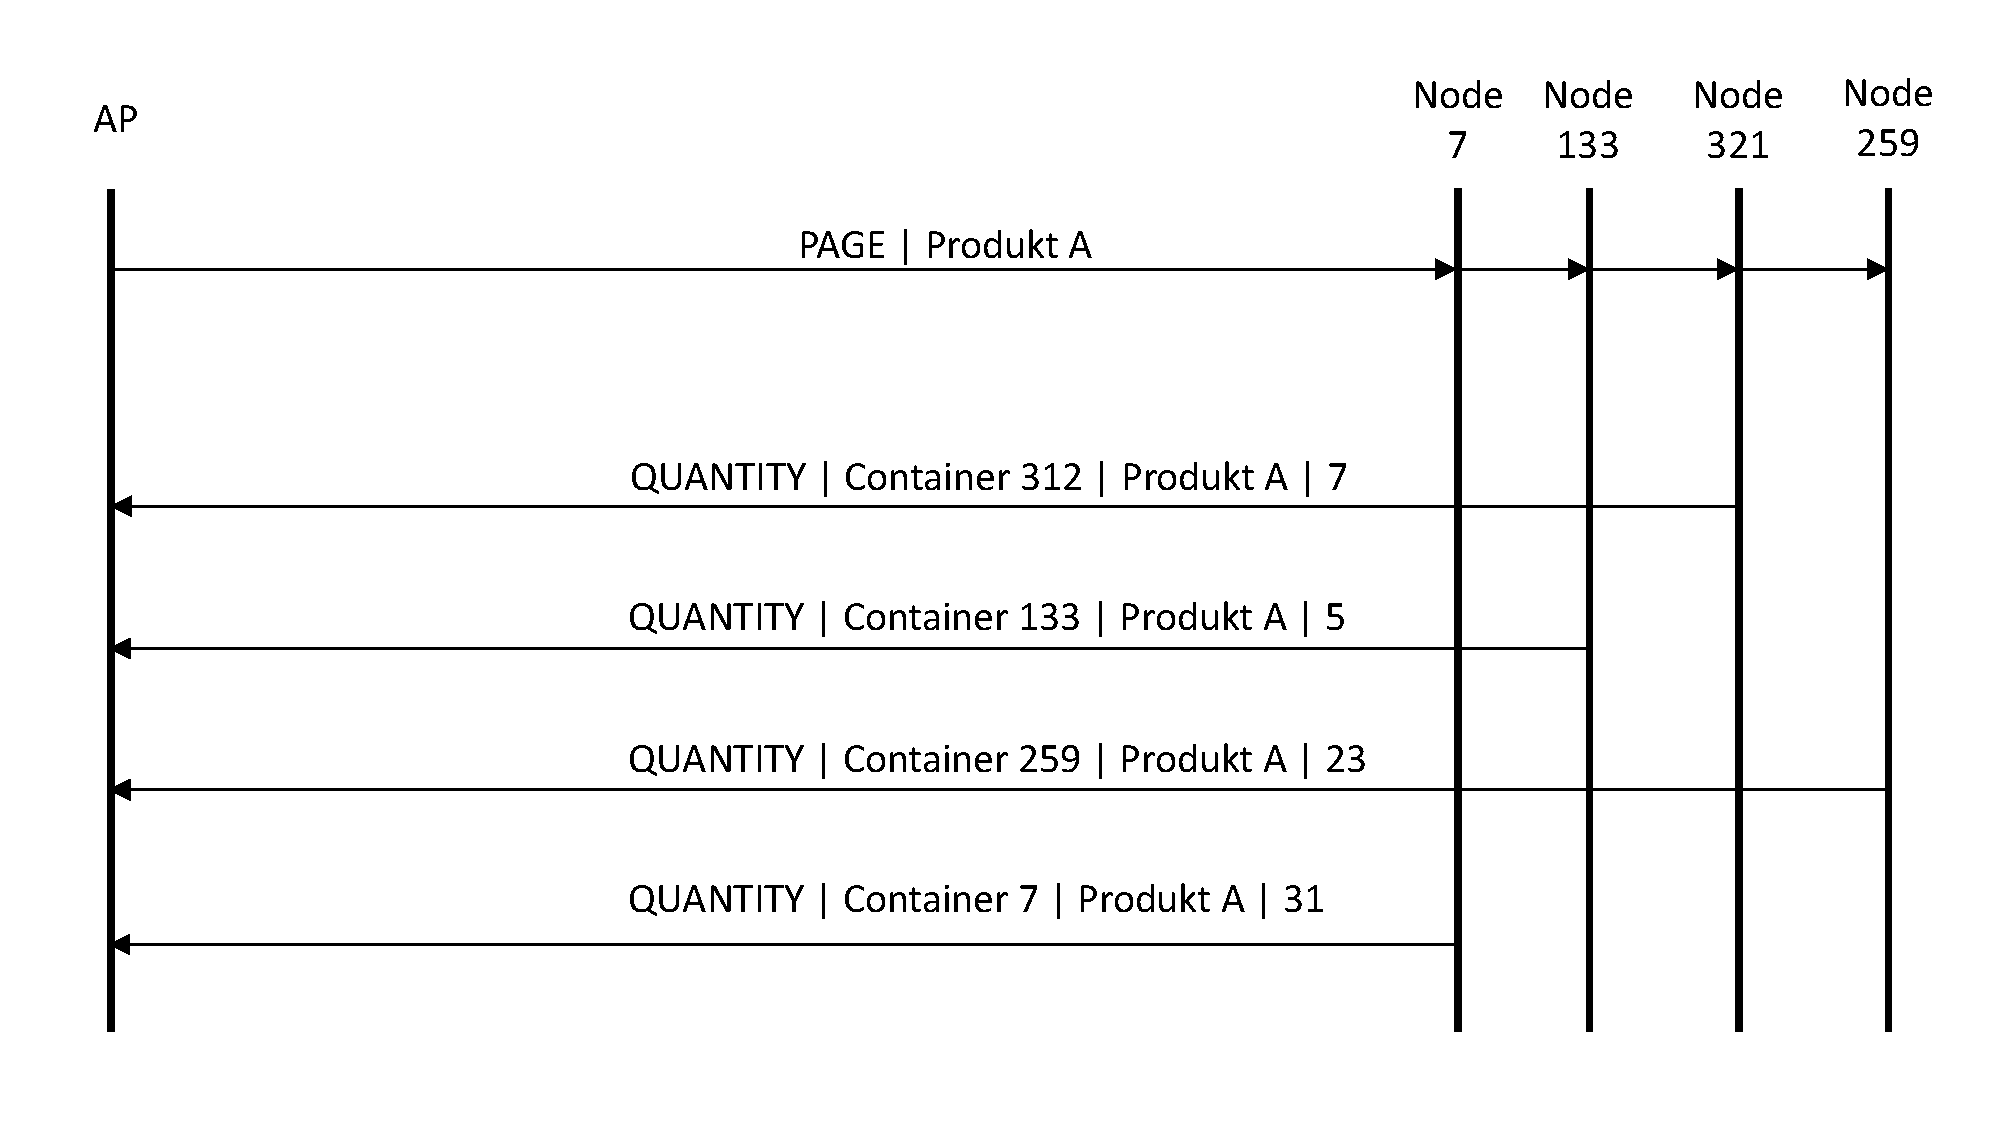
\includegraphics[width=1\linewidth]{gfx/Sequenzdiagramm}} 
        \caption[Sequenzdiagramm]{Sequenzdiagramm der Nachrichten zwischen \acs{ap} und \glspl{node} bei einer Produktanfrage}\label{fig:sequenz}
\end{figure}

Wie in \autoref{kap:verwandtearbeiten} aufgezeigt, sinkt die Leitungsfähigkeit der Systeme in \citep{GreenOrbs} und \citep{inBinTestbed} mit steigender Anzahl an parallelen Vorgängen innerhalb des Netzwerkes. Die Wahl des oben beschriebenen Kommunikationsflusses provoziert diese parallelen Vorgänge durch die hohe Zahl nahezu gleichzeitig versandter \emph{QUANTITY}-Nachrichten und ist daher zur Untersuchung der Kanalzugriffverfahrens geeignet.

Anzumerken ist, dass eine Anfrage über den \ac{ap} immer ein bestimmtes Produkt betrifft. Somit antwortet nur eine Teilmenge der sich insgesamt im Lager befindlichen Frachtcontainer.
Die Ergebnisse dieser Arbeit können daher auch zu einer optimalen Verteilung einer Ware auf Frachtcontainer genutzt werden.


\subsection{Kanalmodell}
Im hier untersuchten Szenario wird als Kanalmodell die Freiraumausbreitung angenommen. 
Eine Analyse mit anderen Kanalmodellen ist zwar nicht Gegenstand dieser Arbeit, die Simulation erlaubt jedoch den Austausch des Kanalmodells für künftige Untersuchungen.

\section{Analyse- und Messmethode}

Ein zentrales Kriterium zur Beurteilung der Leistungsfähigkeit eines Kanalzugriffverfahrens in dem geschilderten Szenario ist die Anzahl an \emph{QUANTITY}-Nachrichten, die nach einer \emph{PAGE}-Nachricht beim \acs{ap} ankommen. Weiterhin ist für die Bewertung der Energieeffizienz des Protokolls der Energieverbrauch an den einzelnen \glspl{node} relevant.
Weiterhin ist die Zeitspanne relevant, nach welcher der \acs{ap} alle Nachrichten empfangen hat. Im Folgenden werden dazu Messgrößen für die Simulation definiert.

\paragraph{Product Specific Delivery Ratio} Die \acf{psdr} bezieht die am \acs{ap} erfolgreich empfangenen Antworten auf die Anzahl der Frachtcontainer mit gleichem Produkt:
\begin{equation}
{r_\textrm{PS}} = \frac{N_\textrm{Antworten}}{N_\textrm{Container mit gleichem Produkt}}
\end{equation}

\paragraph{Mittlerer Energieverbrauch}
.. TODO ..
Bespr. mit Robert, 
passive knoten ausgelassen, da Energieverbrauch unabhängig von Kanalzugriff .. sniffen sowieso nur minimalistisch auf dem kanal

Kanalauslastung

\subsection{Messaufbau}\label{kap:systembeschreibung_sec:analyseaufbau}

\begin{figure}[bth]
        \myfloatalign
        {\includegraphics[width=1\linewidth]{gfx/Analyseaufbau}} 
        \caption[Ananlyseaufbau]{ToDo}\label{fig:sequenz}
\end{figure}

\begin{aenumerate}
\item \emph{PowerScale} System zur Messung des Energieverbrauchs am \gls{node}
\item \emph{Code Composer Studio} Entwicklungsumgebung zur Ausführungssteuerung Prototypenprogramms
\item \emph{Packet Sniffer} Analysesoftware zum Auslesen des CC1200 Funkchips
\item \emph{Real Time Spectrum Analyzer} Messgerät zur kontinuierlichen Anzeige der momentanen Signalstärke im eingestellten Frequenzbereich
\item \emph{hterm} Terminalpraogramm zum seriellen Datenaustausch mit dem \acs{ap}

\end{aenumerate}



%*****************************************
%*****************************************
%*****************************************
%*****************************************
%*****************************************




